\documentclass[11pt]{article}
\usepackage{style/aaai}
\usepackage{times}
\usepackage{url}
\usepackage{latexsym}
\usepackage{color}
\usepackage{bm}
\usepackage{graphicx}
\usepackage{amsmath}
\usepackage{xspace}
\usepackage{multirow}
\usepackage{subfigure}
\usepackage{bbm}
\usepackage{threeparttable}

% new commands for editing
\newcommand{\prob}[2]{\Pr \left( #1 \,|\, #2 \right)}
\newcommand{\mult}[2]{\mathrm{Mult} \left( #1 \,|\, #2 \right)}
\newcommand{\dir}[2]{\mathrm{Dir} \left( #1 \,|\, #2 \right)}
\newcommand{\tabincell}[2]{\begin{tabular}{@{}#1@{}}#2\end{tabular}}
\newcommand{\newcite}[1]{\citeauthor{#1}~\shortcite{#1}}

% commands for text colors
\newcommand{\red}[1]{{\color{red}{#1}}}
\newcommand{\blue}[1]{{\color{blue}{#1}}}
\newcommand{\green}[1]{{\color{green}{#1}}}
\newcommand{\magenta}[1]{{\color{magenta}{#1}}}

% commands for terms
\newcommand{\stlda}{ST-LDA\xspace}
\newcommand{\stlouis}{St.~Louis\xspace}
\newcommand{\obamatalk}{\emph{Obama Talk}\xspace}
\newcommand{\protest}{\emph{Protest}\xspace}
\newcommand{\racism}{\emph{Racism}\xspace}
\newcommand{\curfew}{\emph{Curfew}\xspace}
\newcommand{\michaelbrown}{\emph{Michael Brown}\xspace}
\newcommand{\newsreport}{\emph{News Report}\xspace}
\newcommand{\pray}{\emph{Pray}\xspace}
\newcommand{\shootincident}{\emph{Shoot Incident}\xspace}
\newcommand{\emotion}{\emph{Emotion}\xspace}
\newcommand{\raceandcommunity}{\emph{Race and Community}\xspace}

% commands for comments
\newcommand{\psrcomment}[1]{\textcolor{green}{[PSR: {\bf #1}]} }
\newcommand{\wycomment}[1]{\textcolor{blue}{[WY: {\bf #1}]} }
\newcommand{\lhcomment}[1]{\textcolor{magenta}{[LH: {\bf #1}]} }
\newcommand{\vfmcomment}[1]{\textcolor{red}{[VFM: {\bf #1}]} }

% Use these comment definitions to see paper without comments
%\newcommand{\psrcomment}[1]{}
%\newcommand{\wycomment}[1]{}
%\newcommand{\lhcomment}[1]{}
%\newcommand{\vfmcomment}[1]{}

%\setlength\titlebox{5cm}


\title{Uncovering Topic Dynamics of Social Media and News: A Ferguson Case}

\author{A bunch of new commands are defined. Please take a look at 2016\_icwsm\_topicDynamic.tex.}
%\author{Lingzi Hong \\
%  iSchool \\
%  University of Maryland \\
%  College Park, MD \\
%  {\tt lzhong@umd.edu} \\\And
%  Weiwei Yang \\
%  Computer Science \\
%  University of Maryland \\
%  College Park, MD \\
%  {\tt wwyang@cs.umd.edu} \\\And
%  Philip Resnik \\
%  Linguistics and UMIACS \\
%  University of Maryland \\
%  College Park, MD \\
%  {\tt resnik@umd.edu} \\\And
%  Vanessa Frias-Martinez \\
%  iSchool \\
%  University of Maryland \\
%  College Park, MD \\
%  {\tt vfrias@umd.edu }\\
%}

\date{}

\begin{document}

\maketitle

\begin{abstract}
Looking at the interactions between news content and social media content can help us to understand the increasingly complex dynamics of the relationship between the media and the public surrounding noteworthy news events. Although topic models such as Latent Dirichlet Allocation (LDA) are a valuable tool, they are a poor fit for analyses in which some documents, like news articles, tend to incorporate multiple topics, while others, like tweets, tend to be focused on just one. In this paper, we propose a new model, Single Topic LDA (\stlda), which jointly models news-type documents as distributions of topics and tweets as having a single topic; the model improves topic discovery in news and tweets within a unified topic space by removing noisy topics that conventional LDA tends to assign to tweets in a mixed collection of documents. Using \stlda, we focus on the unrest in Ferguson, Missouri after the fatal shooting of Michael Brown on August 9, 2014, looking in particular at the topic dynamics of tweets in and out of \stlouis area, and at differences and relationships between topic coverage in news and tweets.
\end{abstract}


\section{Introduction}
\label{sec:intro}

Cascading activation model is a widely accepted model, which explores the relationship between government, media and the public~\cite{entman1993framing}. The model helps to explain how frame of information extends down from the White House to elites, media and then to the public of the system. It proposes that moving downward along the cascade is easy, while spreading ideas from lower levels to upper requires extra energy because of the strength of power, the independent environment for decision and comprehensiveness. As the cascade goes down with framing of work from upper layers, the information becomes limited to highlights. The model assumes a certain direction of information flow. Although it acknowledges variation and the possible ways that news feeds back information about the public to influence actions of higher levels, the stair structure emphasizes heavily on the influence from media to the public. However the emergence of social networks makes us think that the situation has changed. 

The creation of social networks aims to provide everyone with equal access to the world, to encourage more independent role in expression, and to achieve information democracy. It has led to increasing participation of information spread, opinion expression and activism by providing easier information access to diverse roles~\cite{kelly2006protest,gonzalez2011dynamics,tufekci2012social}. Social networks become a new competition battlefield for different frames, because everyone can share, comment and create any information. Broader penetration of certain frames becomes more difficult. Politicians even utilize astroturfing, smear campaigns to influence users' choices~\cite{ratkiewicz2010detecting}. On the other side, influence that comes from the public may gain power because they are able to participate and even organize activities online. During the Arab Spring, Twitter has promoted the protest mobilization through reporting real-time event and provided basis for collaboration and emotional mobilization~\cite{breuer2014social}.

It leads us to rethink about the cascade model, specifically on the blurring role of media and users. As a special function role in society, media is still distinctive, but information spreading between media and the public is in both directions, so we want to study whether the power of influence is blurred for media and the public. The following two questions are emphasized:

\begin{enumerate}
\item Is the public still heavily influenced by frames of the media?
\item Does the media pay attention to what the public concerns and reflect the voice from the public?
\end{enumerate}

The influence is hard to detect, considering the difficulty of capturing the status of the public before and after media news. However, we can study the topics of users and media and how these topics are related in time series, as an evidence of media coverage of the public opinions, or influence of media on users.  

In this study, we take Ferguson unrest event in 2014 as an example, to analyze news and tweets topics along with the evolvement of the case. Based on latent Dirichlet allocation~\cite[LDA]{blei2003latent}, Single Topic LDA (\stlda) is proposed to bring long news documents and short tweets under a unified topic frame, so that topics of news and tweets are comparable. From intuition, we assume that long news documents are comprised with multiple topics, while each tweet has only one topic because of the length limitation. Then daily distribution of topics of news and tweets are compared. We also analyze the difference of topics in geography, hypothesizing that geographical culture congruency may lead to different focuses of the public and thus various reactions to media topics.

The contribution of this study lays in three main aspects. First, we tackle the technical problem of building topic model for a mixture of short and long documents. Conventional topic models such as LDA and PLSA~\cite{hofmann1999probabilistic} perform badly on because co-occurrence patterns in short texts are sparse. Consider a tweet with 5 words, every word's topic assignment makes up 20\% of its topic proportion, but usually a tweet's main topic is decided by 2 or 3 words. In this case, the main topic proportion is about 40\% to 60\%, which does not reflect the truth. Our model considers the words in a tweet as a whole and assigns only one topic to a tweet, so that the main topic is more likely to be assigned.
Second, this preliminary study offers a method to understand which are strong frames, which has been a challenge for social scientists~\cite{chong2007framing}. By examining the topic dynamics between news and social media, which are separately representative of media and the public, we may understand which news is influential or which frames are more competitive by analyzing opinions of the public.
Third, bringing tweets and news to the same topic frames will help us to understand large volumes of tweets through news, thus in a more understandable way. When training topic models separately on news and tweets, it is not easy to understand how topics in news and tweets match each other. When combining tweets and news together for analysis, on the other hand, the latent meaning of a topic is the same for tweets and news. Thus large amount of tweets can be represented by news with similar topic distribution, which makes it easier to know public opinions and estimate for opinion poll. 


\section{Related Work}
\label{sec:related_work}

We aim to study the interaction between media and the public by studying dynamics of news and tweets topics during the Ferguson unrest event. The most related research topics are agenda setting online. Political social scientists have noticed the change brought by Internet.~\newcite{sayre2010agenda} propose the question of roles and agenda setting form in the digital age. They manually analyze thousands of videos and news media on Proposition 8 in California, and find that post content in open social media reflects mainstream news, while posts also have influence on professional media coverage, thus create opinion dynamics. The results innovatively reveal the relationship between media and the public in a descriptive way. However it needs large amount of human efforts to apply this method to other events, and it is hard to identify the weight change of topics during the evolving process.

Topic detection has been widely studied for news and social media. Tracking of memes on the Internet is a way to understand dissemination of certain information content. Memes are entities that represent units of information at the desired level of detail~\cite{ratkiewicz2010detecting}. The semantic units play as clear clues for detecting dynamic change of diverse topics.~\newcite{leskovec2009meme} introduce a meme-tracking technique and use it to track topic shifts in news and blogs over a long time. They observe a 2.5-hour lag between peaks of attention to a phrase in the news media and in blogs, which shows evidence of possible interaction between media and other individuals. It involves tracking of repeating semantic entities, as a way for topic tracking, but according to the algorithm only repeated topics, thus memes, can be detected. Entity extraction is also a way to track information diffusion on the Internet.~\newcite{kim2012event} extract 5W1H (\emph{Who}, \emph{What}, \emph{Where}, \emph{When}, \emph{Why} and \emph{How}) structure from events and detect the connection between news, blogs and social networking in a supervised way. However entity expression is limited to specific events rather than topics or frames.

As a big collection of crowding sourcing opinions, tweets have been studied a lot to understand public opinions in social events such as the 2011 Tunisian and Egyptian Revolutions~\cite{gonzalez2011dynamics}, information sharing in protest during the G20 meetings in 2009~\cite{earl2013protest}, and organization of movement in the Occupy Wall Street protest~\cite{conover2013geospatial}. These studies focus more on information flow between different roles rather than the evolving of topics. Topic detection in tweets has been studied because there is challenge for the short length of texts~\cite{yan2013biterm,zhao2011comparing}.

Aggregating short tweets into long document units is a way to alleviate the problem, such as author-based aggregation which is used to identify user topics and measure user similarity~\cite{weng2010twitterrank}. Aggregation based on time slices is used to track emerging events in Twitter~\cite{lau2012line}.~\newcite{hong2010empirical} also propose a method to aggregate tweets by similar words, which tend to work better than regular LDA. However the performance of these methods depends much on the research question and available datasets.

Other variations of topic model are proposed to discover topics from tweets. Biterm topic model~\cite[BTM]{yan2013biterm} directly simulates the generation of word co-occurrence patterns in corpus, thus enhances learning and leads to more coherent topics. A similar model is Word Network Topic Model~\cite{zuo2014word}, which also utilizes word co-occurrence network to solve the sparsity problem.~\newcite{zhao2011comparing} propose a Twitter-LDA model, which assumes that a single tweet is usually about a single topic, to discover topics from a representative sample of the entire Twitter. Supervised methods have also been applied to find tweets topics, such as Labeled-LDA~\cite{ramage2009labeled}, which maps the content of the tweets into dimensions of substance, style, status and social characteristics~\cite{ramage2010characterizing}.

There are studies working on alignment of events information and tweets, which are similar to our work.~\newcite{hu2012lda} propose a joint Bayesian model for events transcripts and tweets, which supposes that event information can impost topical influence on tweets.~\newcite{gao2012joint} create a joint topic model to extract important and complementary pieces of information across news and tweets, and generate complimentary information from both. These models infer tweets topics incorporating information from event transcripts or news. So tweets and event or news topics are under a unified frame. The difference is that, in our method, each tweet is treated to have one topic instead of a probability of distribution of topics. We bring news and tweets together for training, and prove that \stlda model performs better for discovery of topic dynamics.


\section{Methodology}
\label{sec:model}

\subsection{Single Topic LDA Model}

We propose \stlda to deal with short documents like tweets and long documents like news simultaneously. The intuition is that short documents are unlikely to be related to multiple topics. Instead, one short document is usually talking about a single topic and all its words are generated from this topic. Meanwhile, long documents still follow conventional LDA assumptions: each document contains a mixture of topics. Specifically, the generative process of tweets and news is defined as

\begin{enumerate}
\item For each topic $k \in \{1, \ldots, K\}$
    \begin{enumerate}
    \item Draw word distribution $\bm{\phi_k} \sim \mathrm{Dir}(\beta)$
    \end{enumerate}
\item For each news document $d\in \{1, \ldots, D^\mathrm{N}\}$
    \begin{enumerate}
    \item Draw topic distribution $\bm{\theta^{\mathrm{N}}_{d}} \sim \mathrm{Dir}(\alpha)$
    \item For each token $t^{\mathrm{N}}_{d,n}$ in news document $d$
        \begin{enumerate}
        \item Draw a topic $z^{\mathrm{N}}_{d,n} \sim \mathrm{Mult}(\bm{\theta^\mathrm{N}_d})$
        \item Draw a word $w^{\mathrm{N}}_{d,n} \sim \mathrm{Mult}(\bm{\phi_{z^{\mathrm{N}}_{d,n}}})$
        \end{enumerate}
    \end{enumerate}
\item Draw tweet background topic distribution $\bm{\theta^{\mathrm{T}}} \sim \mathrm{Dir}(\alpha)$
\item For each tweet document $d \in \{1, \ldots, D^\mathrm{T}\}$
    \begin{enumerate}
    \item Draw a topic $z^{\mathrm{T}}_d \sim \mathrm{Mult}(\bm{\theta^{\mathrm{T}}})$
    \item For each token $t^{\mathrm{T}}_{d,n}$ in document $d$
        \begin{enumerate}
        \item Draw a word $w^{\mathrm{T}}_{d,n} \sim \mathrm{Mult}(\bm{\phi_{z^{\mathrm{T}}_d}})$
        \end{enumerate}
    \end{enumerate}
\end{enumerate}

The corresponding graphical model is given in Figure~\ref{fig:stlda}.

\begin{figure}[h]
\centering
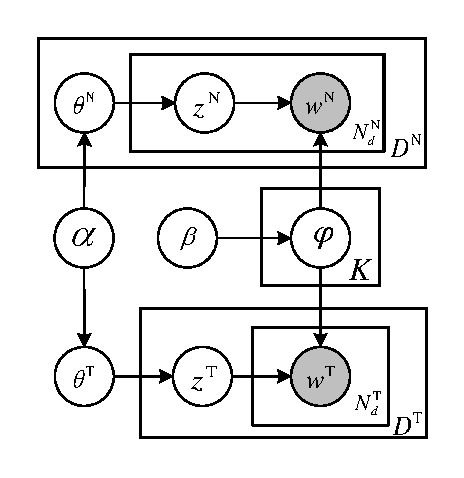
\includegraphics[width=.8\linewidth]{figures/stlda_model.pdf}
\caption{Graphical Model of \stlda}\label{fig:stlda}
\end{figure}

The model's news part is the same as that of conventional LDA, but its tweet part is different.
Specifically, the coverage of two plates are different, which is adapted according to our assumptions.

The first difference is the coverage of word plate (the one with subscript $N^\mathrm{T}_d$).
In LDA, it covers both $\bm{z}$ and $\bm{w}$, denoting that every word has its own topic assignment and every document consists of a mixture of topics.
In \stlda's tweet part, the plate only covers $\bm{w}$, which means that every word in a tweet is generated from the same topic.\psrcomment{Is there going to be a problem with ``generic" or ``non-topical" words? Not \emph{every} content word is topical, is it?}\wycomment{``Non-topical" words are of almost the same probability to be assigned to each topic. They won't lead the tweet to a wrong topic if they do not dominate the tweet.}

The second difference is the coverage of document plate (the one with subscript $D^\mathrm{T}$). LDA assumes that every document has a topic distribution, but in \stlda, every tweet only has one topic which can not form a distribution inside a document. Thus, $\bm{\theta^\mathrm{T}}$ is outside the document plate and denotes a background topic distribution of tweets.

\subsection{Posterior Inference}
The posterior inference of \stlda can be done by Gibbs sampling. The sampling equation for news documents is the same as conventional LDA. The probability of $n$-th token in news document $d$ being assigned to a topic $k$ is computed as

\begin{align}
&\prob {z_{d,n}=k} {\bm{z_{-d}},\bm{w_{-d,n}},w_{d,n}=v} \notag\\
\propto &\left( N_{d,k}^{-d,n} + \alpha \right) \frac {N_{k,v}^{-d,n} + \beta } {N_{k,\cdot}^{-d} + V\beta},
\end{align}
where $N_{d,k}$ denotes the number of tokens in document $d$ assigned to topic $k$; $N_{k,v}$ denotes the count of word $v$ assigned to topic $k$. Marginal counts are denoted by $\cdot$. $^{-d,n}$ denotes that the count excludes the $n$-th token in document $d$.

The probability of tweet $d$ being assigned a topic $k$ is computed as

\begin{align}
&\prob {z_d=k} {\bm{z_{-d}},\bm{w}} \notag\\
\propto &\left( N_k^{-d} + \alpha \right) \frac {\prod\limits_{v=1}^{V} \prod\limits_{i=0}^{N_{d,v}-1} \left( N_{k,v}^{-d} + \beta + i \right)} {\prod\limits_{i=0}^{N_{d,\cdot}-1} \left( N_{k,\cdot}^{-d} + V\beta + i \right)},
\end{align}
where $N_k$ denotes the number of documents assigned to topic $k$; $N_{d,v}$ is the count of word $v$ in document $d$. $^{-d}$ denotes that the count excludes document $d$.

%A brief derivation of Gibbs sampling equation is attached in %Appendix~\ref{sec:derivation}.

% After we train a model on training corpus, we can apply it on unseen documents and infer their topic assignments. The Gibbs sampling equation for test is much simpler. The probability of assigning topic $k$ to document $d$ is

% \begin{equation}
% \prob {z_d=k} {\bm{z_{-d}},\bm{w_d}} \propto \left( N_k^{-d} + \alpha \right) \prod_{v=1}^{V} \phi_{k,v}^{N_{d,v}}.
% \end{equation}

\subsection{Topic Dynamics}
\stlda is able to train long (news) and short documents (tweets) simultaneously, by assigning multiple topics to long documents and one topic to short documents.\psrcomment{This is the generative process for \emph{tweets}, but what about news? If this is the whole model, how do news stories get multiple topics?}\wycomment{Yes, I've updated the model.}
The output results of \stlda model can be used for further discovery of topic dynamics of tweets and news.
We define topic dynamics as temporal change of topics using daily sliding window.
Assuming that every news document has the same impact and contributes equally to the total media environment,\psrcomment{A big assumption? Add weighting?} the topic proportion of day $t$ is the average of topic probabilities of all news documents on that day as

\begin{equation}
\bar{\theta}_{t,k}^{\mathrm{news}}=\frac{\sum_{d=1}^{D_t^{\mathrm{news}}} \theta_{d,k}}{D_t^{\mathrm{news}}},
\end{equation}
where $D_t^{\mathrm{news}}$ denotes the number of news documents on day $t$; $\theta_{d,k}$ is topic $k$'s proportion in document $d$.

Differently, each tweet $d$ has only one topic $z_d$ given by \stlda. Under the same assumption that each tweet contributes equally to the voice of public, the aggregation of daily tweet topic proportion is calculated as

\begin{equation}
\bar{\theta}_{t,k}^{\mathrm{tweets}} = \frac{\sum_{d=1}^{D_t^{\mathrm{tweets}}} \mathbbm{1}(z_d=k)}{D_t^{\mathrm{tweets}}},
\end{equation}
where $D_t^{\mathrm{tweets}}$ denotes the number of tweet documents on day $t$ and $\mathbbm{1}(\cdot)$ is an indicator function.

Given $\bm{\bar{\theta}_t^{\mathrm{news}}}$ and $\bm{\bar{\theta}_t^{\mathrm{tweets}}}$ where $t$ varies from August 11 to 27, we can identify topic dynamics by the changing of daily topic proportions. 

\section{Dataset}
\label{sec:dat}

We collected 13,238,863 tweets from August 10, 2014 to August 27, 2014 mentioning Ferguson using the Twitter Streaming API.
Among them 92,184 are geo-tagged, which takes about 0.70\% of all.
We use geo-tagged tweets instead of all tweets because an empirical study~\cite{he2015uncovering} shows that there is geographic difference in tweet topics for a certain event.\psrcomment{It would be interesting to see what it looks like if all 13.2M tweets are used.}
Meanwhile there is not much difference in the reaction time, volume, and topics between geo-tagged tweets and non geo-tagged tweets.
So we use geo-tagged tweets to analyze topics in different areas, in representative of general public opinions.
To assist geographic analysis, we use 2014 TIGER/Lines Shapefile to identify the locations of tweets according to tweets' coordinates.\footnote{\url{https://www.census.gov/geo/maps-data/data/tiger-line.html}}

News is crawled by the links published by news account on Twitter. We randomly selected 108 media accounts from Twitter, for example ``Washington Post", ``NBC News" and ``ABC7News", collected all the tweets they published during the Ferguson event, and extracted news reports from the links they published. In total, there are 1,338 news covering from August 11 to 27.

Same standard preprocessing procedure is applied to news and Twitter corpora, such as tokenization, POS tagging, lemmatization, bigrams detection, stop words, low frequency words and too high frequency words removal. However, we use different tools for the two corpora: OpenNLP package~\cite{baldridge2005opennlp} for news corpus and Tweet NLP package~\cite{owoputi2013improved} for Twitter corpus. After preprocessing and removing empty documents, there are 1,275 news documents and 81,553 Twitter documents, as well as a vocabulary with 1,132 words.









\section{Evaluation of Topic Quality}
\label{sec:eva}

In this section, we compare the performance by evaluating the topic quality given by LDA and \stlda both intrinsically and extrinsically. The hyperparameters $\alpha$ and $\beta$ are both set to 0.1 and the number of topics is set to 10.

As topics given by two models are in different orders, we match the topics based on KL divergence before comparing them. The matching procedure starts by obtaining a KL divergence table $T$. Each cell $T_{k_1,k_2}$ stores the KL divergence of topic $k_1$ given by LDA and topic $k_2$ given by \stlda as

\begin{eqnarray}
T_{k_1,k_2}&=&\mathrm{KL}(\bm{\phi_{k_1}^\mathrm{LDA}}||\bm{\phi_{k_2}^\mathrm{\stlda}})\\
&=&\sum_{v=1}^{V} \phi_{k_1,v}^{\mathrm{LDA}} \log_2 \frac{\phi_{k_1,v}^{\mathrm{LDA}}}{\phi_{k_2,v}^{\mathrm{\stlda}}}.
\end{eqnarray}

Then we run a depth-first search algorithm on the KL divergence table to find the best match which has the smallest the overall KL divergence.\psrcomment{C.f. Hungarian Algorithm for bipartite graph matching.}

\subsection{Comparison of Topics}

\begin{table*}[htpb]
\centering
\begin{threeparttable}
\begin{tabular}{|c|c|l|}
\hline
\bf \tabincell{c}{Model\\(Corpus)} & \bf Topic & \multicolumn{1}{c|}{\bf Top Words}\\ \hline
\multirow{5}*{\tabincell{c}{LDA\\(NT)\tnote{1}}} & Obama Talk & \tabincell{l}{happen, i'm, make, thing, talk, situation, what's, what's\_happen, bad, you're\\\psrcomment{Not clear how label and words are connected}\\\wycomment{It seems so. Lingzi, could you please double check?}}\\ \cline{2-3}
 & Protest & tear\_gas, protester, arrest, fire, medium, rt, protestor, street, crowd\\ \cline{2-3}
 & Racist & black, white, loot, protect, community, racist, stop, race, citizen, riot\\ \cline{2-3}
 & Curfew & missouri, state, obama, national\_guard, call, curfew, mo, press, governor\\ \cline{2-3}
 & Pray & peace, pray, justice, stand, love, tonight, hope, stay, family, safe\\ \hline
\multirow{5}*{\tabincell{c}{\stlda\\(NT)}} & Obama Talk & obama, president, law\_enforcement, house, holder, make, story, post, include\\ \cline{2-3}
 & Protest & tear\_gas, arrest, protester, fire, rt, reporter, medium, shoot, crowd\\ \cline{2-3}
 & Racist & black, white, make, race, america, obama, stop, happen, situation, riot\\ \cline{2-3}
 & Curfew & missouri, curfew, state, national\_guard, governor, nixon, call, gov, order\\ \cline{2-3}
 & Pray & peace, pray, stand, justice, night, love, tonight, today, family\\ \hline
\multirow{5}{*}{\tabincell{c}{LDA\\(N)\tnote{2}}} & Obama Talk & obama, president, house, make, white, news, national, deal, run, defense\\ \cline{2-3}
 & Protest & st\_louis, nixon, protester, shooting, county, justice, aug., investigation, state, thursday\\ \cline{2-3}
 & Racist & black, make, white, cop, time, don't, year, good, man, thing\\ \cline{2-3}
 & Curfew & protester, johnson, tear\_gas, crowd, curfew, night, fire, street, missouri, shoot\\ \cline{2-3}
 & Pray & (No matching topic)\\ \hline
\end{tabular}
\begin{tablenotes}
\footnotesize
\item[1] NT: news and tweets.
\item[2] N: news only.
\end{tablenotes}
\caption{Topic Examples}\label{tab:topic}
\end{threeparttable}
\end{table*}

To evaluate topic quality, we select the top words under each topic. Because news and tweets are trained together with imbalanced number of documents, it is possible that both models may be biased for one type of documents, thus topics may come from only news or tweets. To ensure that both LDA and \stlda have balanced topics that come from tweets and news, we train another model merely on news and set the results as a baseline for comparison.

Table~\ref{tab:topic} shows four common topics for all three models and one topic that only exists in results trained on news and tweets together. Four common topics indicate that news topics are kept when mixture of documents are trained together. But for the one topic \pray, there is no matching topic in results of LDA on news, which tends to be the topic that only exists in tweets. It is also worth noting that top words in the four common topics are different. Top words in LDA on news tend to be more complicated and in written language style, such as \emph{justice} and \emph{investigation}. But top words in the topics by mixture texts are a little different. There are oral phrases, such as \emph{i'm} and \emph{you're}, and words which are highly probable to come from tweets such as \emph{rt} and \emph{gov}. These Twitter words indicate that such topics are also covered by tweets. So we can conclude that \stlda can extract topics from both tweets and next, not biased to one type of texts, and it discovers topics that are common in both news and tweets. However, according to analysis of coverage of topics and top words, there is not much difference between LDA and \stlda. It just verifies that there is not extreme bias for either type of texts when trained together. In Section~\ref{subsec:intrinsic}, we evaluate the quality of tweets' topics as an intrinsic evaluation. Extrinsic evaluation is applied in Section~\ref{subsec:extrinsic}, by using two models in discovery of topic dynamics.

\subsection{Topic Quality for Tweets}
\label{subsec:intrinsic}

To examine the quality of topic assignment, the most intuitive way is to pick a document and see whether the topic distribution is reasonable to represent the content. Because news is long and contains mixture of latent topics, it is hard to decide whether the topic distribution is appropriate. On the other hand, a tweet is usually constituted by one or two sentences, so it is intuitive to evaluate whether the topic assignment is appropriate.

We list five tweets in Table~\ref{tab:tweets} and their topic distributions by LDA and topic assignments by \stlda are given in Table~\ref{tab:tweet_topic}. Topics in LDA and \stlda are matched and numbered from 0 to 9. Topic names are manually summarized according to top frequency words in the topic.

\begin{table*}[htpb]
\centering
\begin{tabular}{|c|c|p{13cm}|}
\hline
\bf No. & \bf Label & \multicolumn{1}{c|}{\bf Content}\\ \hline
1 & News/Pray & ``@bkesling: ``Hands up, don't shoot" after tear gas fired in \#Ferguson http://t.co/9zQIh31wQg" modern day America...  \#PrayForFerguson\psrcomment{Label: News? Prayer?}\\ \hline
2 & Race & 80\% black folks think \#Ferguson raises ``important issues about race that need to be discussed," only 37\% of white folks do. Very sad.\psrcomment{Label: Race}\\ \hline
3 & Sarcastic Police & You guys can't blame that cop in \#Ferguson. Shooting your gun 6 times is literally the answer to every question in their training manual.\psrcomment{Label: Sarcastic police/race}\\ \hline
4 & Protest & \#fergusongate media get it straight. U act like those who don't live in ferguson can't protest. This is for all blacks everywhere.\psrcomment{Label: Protest}\\ \hline
5 & News & But thank God for social media though. Imagine if we're dependent on the news to tell the ``truth" about what's really happening in \#Ferguson\psrcomment{Label: News}\\ \hline
\end{tabular}
\caption{Tweet Examples}\label{tab:tweets}
\end{table*}

\begin{table*}[htpb]
\centering
\begin{tabular}{|c|c|c|c|c|c|c|c|}
\hline
\multicolumn{3}{|c|}{\bf Tweets} & 1 & 2 & 3 & 4 & 5\\ \hline
\multirow{10}{*}{\tabincell{c}{\bf LDA Topic\\ \bf Distribution}} & 0 & Obama Talk & 0.017 & \bf 0.373 & 0.011 & 0.017 & \bf 0.888\\ \cline{2-8}
 & 1 & Protest & \bf 0.517 & 0.009 & 0.011 & \bf 0.183 & 0.013\\ \cline{2-8}
 & 2 & Racism & 0.017 & \bf 0.555 & \bf 0.233 & 0.017 & 0.013\\ \cline{2-8}
 & 3 & Curfew & 0.017 & 0.009 & 0.011 & 0.017 & 0.013\\ \cline{2-8}
 & 4 & Michael Brown & 0.017 & 0.009 & \bf 0.567 & \bf 0.183 & 0.013\\ \cline{2-8}
 & 5 & News Report & 0.017 & 0.009 & 0.011 & 0.017 & 0.013\\ \cline{2-8}
 & 6 & Pray & 0.017 & 0.009 & 0.011 & 0.017 & 0.013\\ \cline{2-8}
 & 7 & Shoot Accident & \bf 0.350 & 0.009 & 0.011 & 0.017 & 0.013\\ \cline{2-8}
 & 8 & Emotion & 0.017 & 0.009 & \bf 0.122 & \bf 0.183 & 0.013\\ \cline{2-8}
 & 9 & Race and Community & 0.017 & 0.009 & 0.011 & \bf 0.183 & 0.013\\ \hline
\multicolumn{3}{|c|}{\bf \stlda Topic} & 1 & 2 & 4 & 8 & 5\\ \hline
\end{tabular}
\caption{Tweet Topic Comparison}\label{tab:tweet_topic}
\end{table*}

The first tweet talks about the conflict between protesters and the police, with a description of the situation and a short comment.
It is assigned with two topics with relatively high probability by LDA, thus \protest and \shootincident.\psrcomment{I think you mean \emph{Incident}.}\wycomment{I guess so. I've updated all ``Shoot Incident". If it should be ``Shoot Accident", just modify the command.}
Words in \shootincident talks about \emph{shoot}, \emph{Michael\_brown} and \emph{street}, which tend to be description of the shoot accident.
Although the sentence contains words like \emph{shoot}, it is not appropriate to be assigned with topic 7.
Meanwhile for the tweet there is small probability under other topics such as \obamatalk and \racism, which have nothing to do with the content of the tweet.
Similarly the second tweet mainly talks about racism, which is what \stlda gives.
But it also has the latent topic \obamatalk with probability 0.373, and a slight probability for other topics under LDA model. From the text of tweet, it is neither relevant to \obamatalk, nor to other topics.
The third tweet is talking about police shooting at Michael Brown, which is closest to topic about the accident, so topic 4 \michaelbrown is appropriate, but others are not.
The common pattern in these three cases is that the topic with highest probability in LDA is consistent with the topic given by \stlda.
Is it true for all tweets? Could we just use LDA and assign tweet with the one topic with highest probability?

The case of 4th tweet is slightly different. The 4th tweet is constituted by 3 sentences, which seem to talk about media, the protest and race issues. The tweet is assigned by LDA with 5 topics with equally high probability, thus \protest, \michaelbrown, \shootincident, \emotion and \raceandcommunity. However it seems that the tweet doesn't mention Michael Brown accident, or shooting things. Similar with the three cases above, there are noisy topics in results given by LDA. It assigns part of the probability to wrong topics, which makes the right topic not so significant. This is the shortage of LDA but tackled by \stlda.
The 5th tweet shows how \stlda assigns the right topic but LDA fails to. The tweet talks about the role of social media in contrast with news media. The topic is mainly about how others describe the event. So topic 5 \newsreport is appropriate. However, the highest probability goes to \obamatalk by LDA, which is not relevant.

The analysis of tweets shows that \stlda has advantage in assigning tweets with one topic, because most of the tweets are short and actually contain only one topic. LDA gives each tweet a probability distribution of topics, which usually contains irrelevant topics and also decreases the importance of right topic. Meanwhile the results of \stlda can't be substituted by assigning the topic with highest probability in the distribution.

\subsection{Comparison of LDA and \stlda in Topic Dynamics}
\label{subsec:extrinsic}

The extrinsic evaluation is conducted to see how the two algorithms perform in showing topic dynamics. We compare the results of topic dynamics in news and tweets. Figure~\ref{fig:news_topics} shows the change of news topic proportions from August 11 to 27 based on the results of LDA and \stlda. It is similar that investigation of shoot accident and discussion of race are the two main themes of news. Along with the evolvement of event, the proportion of race issues increases, while the voice of investigation reaches a peak on August 17 and decreases thereafter.

\begin{figure*}[htpb]
\centering
\subfigure[LDA]
{
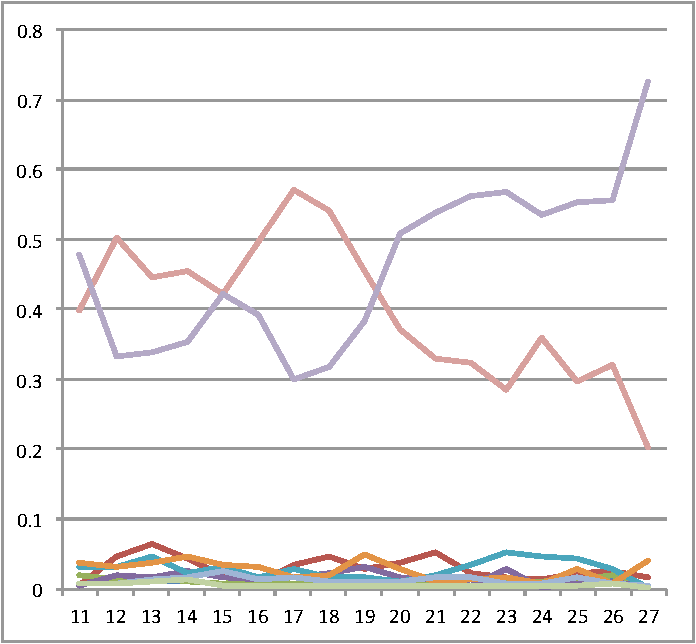
\includegraphics[width=0.48\linewidth]{figures/1LDANews-2.pdf}
\label{fig:news_topics_lda}
}
\subfigure[\stlda]
{
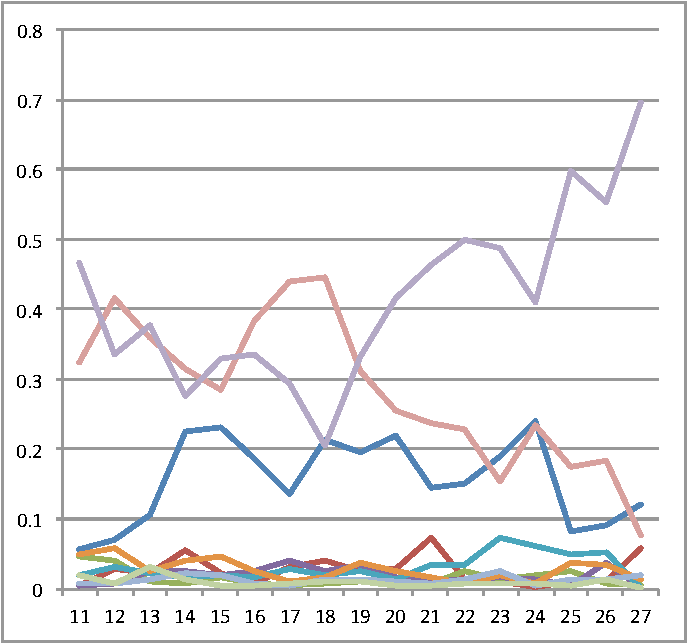
\includegraphics[width=0.48\linewidth]{figures/1STLDANews-2.pdf}
\label{fig:news_topics_stlda}
}
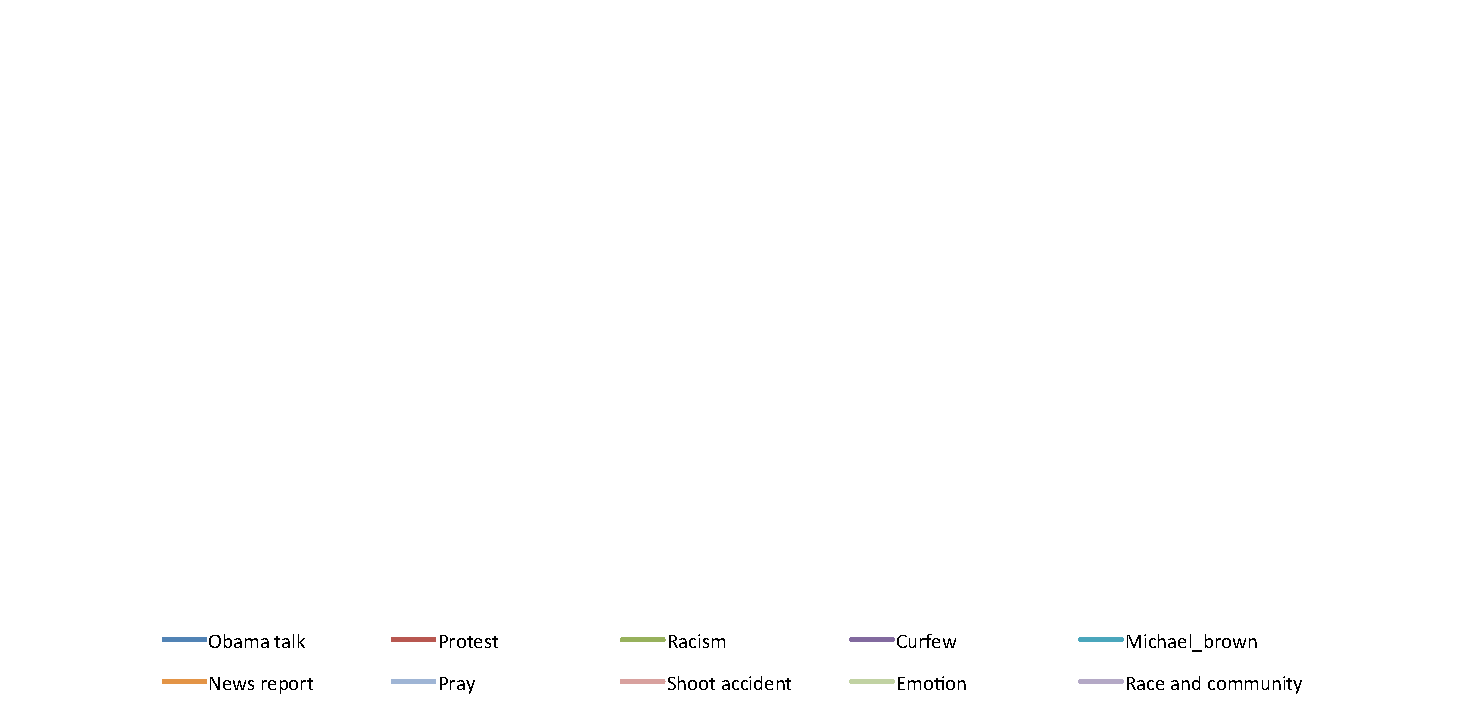
\includegraphics[width=\linewidth]{figures/Legend.pdf}
\caption{News Topic Dynamics by LDA and \stlda}\label{fig:news_topics}
\end{figure*}

Topic distribution given by LDA is highly skewed to two main topics, thus the \shootincident and the \raceandcommunity, while other topics take only a small proportion and it is hard to identify the proportion change of these topics. Meanwhile \stlda gives results that are slightly better in representing different topics. Besides the significant change of \shootincident and \raceandcommunity, the \obamatalk is discovered as a main topic for media. It keeps a relatively stable proportion of 20\%, and peaks after some important events related with Obama. For example, on August 12, Obama addressed the shooting and urged the community in Ferguson to stay calm. On August 14, he gave a talk saying there is no excuse for protesters to turn to violence, which seems to lead to the peak on August 14 and 15. Also in news topic dynamics by \stlda, the \protest shows a peak on August 21, which is consistent with the date when the National Guard withdrew from the Ferguson.

Both LDA and \stlda are unsupervised methods, so it is hard to verify which topic dynamic reflects the real situation. But the topics discovered by \stlda are more diverse, and are consistent with the important events in the timeline.

There is more variance in topic dynamics of tweets by \stlda than LDA, which is shown in Figure~\ref{fig:tweets_topics}. The proportion of topics is close to each other in topic dynamics by LDA, so it is relatively hard to identify the main topics for each day. There is rising point of \michaelbrown after the shoot accident, and a peak on August 25 when the funeral for Michael Brown is held. However, consistent with the shortage discussed in analysis of tweet topics, LDA gives a probability distribution of topics, of which some are irrelevant. So when aggregating tweets in a day together, the proportion number for each topic is similar, which makes it hard to identify main topics on that day, and change of topics along the time. Comparatively, \stlda gives results with better representation of topic dynamics. There is variation of topics changing overtime. It is clearly that after the shoot accident, emotion of the public surges to a peak on August 11. After the protest event, another emotion topic appears on August 14. Meanwhile, the proportion of \pray topic keeps relatively stable from August 11 to August 24, and increases a lot on the day when Michael Brown's funeral is held. These tendencies in topic changes can be seen in topic dynamics of tweets by LDA, but these topics are entangled with other topics, making it hard to differentiate from other topics.

\begin{figure*}[htpb]
\centering
\subfigure[LDA]
{
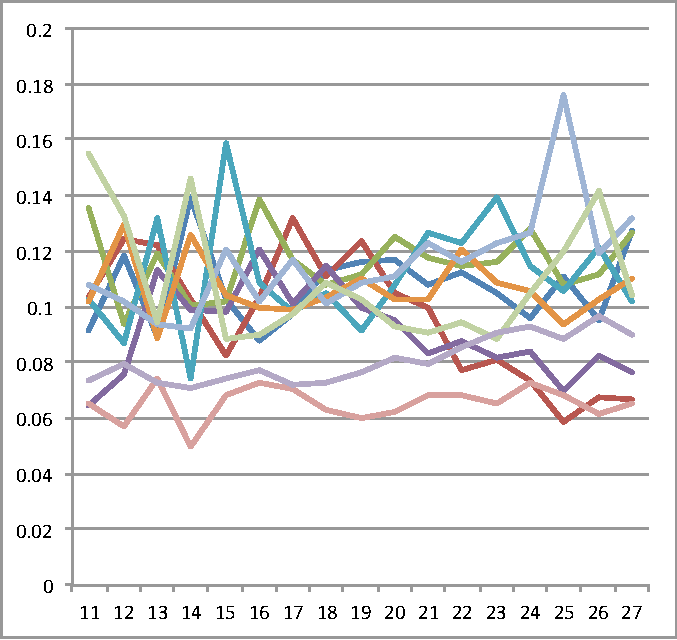
\includegraphics[width=0.48\linewidth]{figures/2LDATweets.pdf}
\label{fig:tweets_topics_lda}
}
\subfigure[\stlda]
{
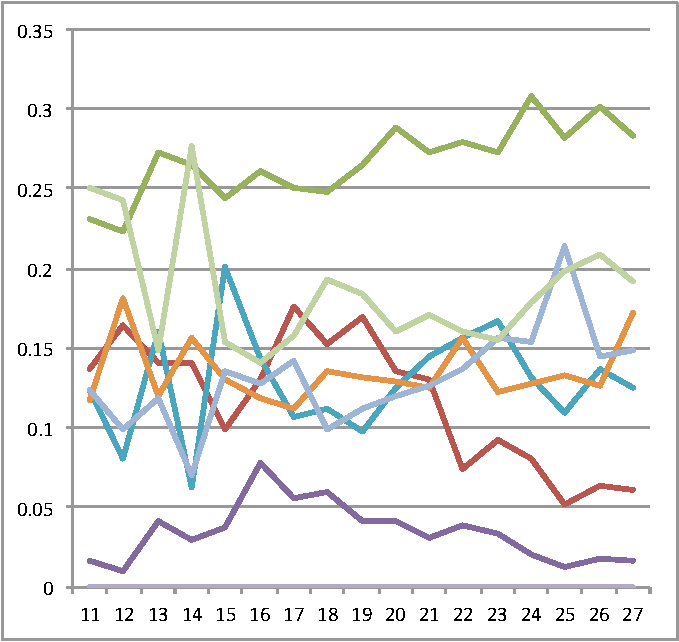
\includegraphics[width=0.48\linewidth]{figures/2STLDATweets.pdf}
\label{fig:tweets_topics_stlda}
}
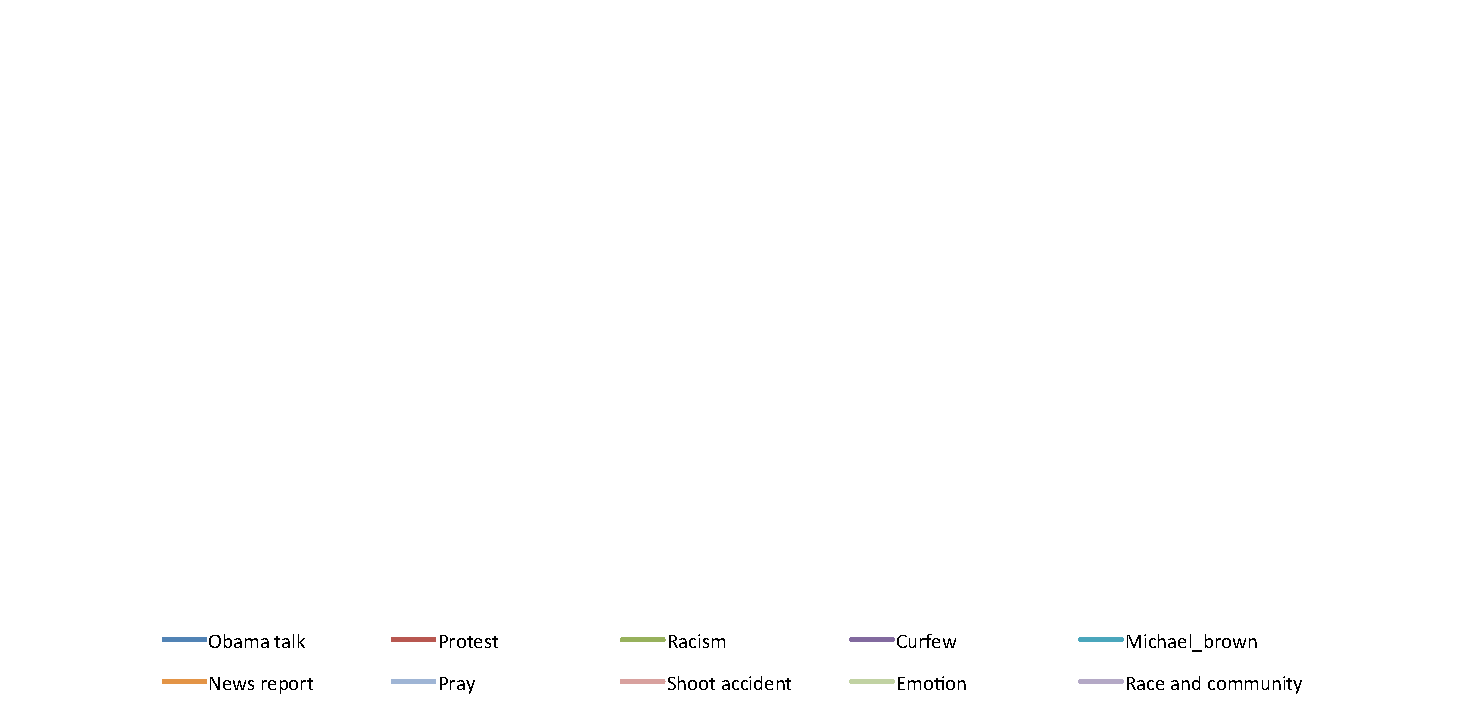
\includegraphics[width=\linewidth]{figures/Legend.pdf}
\caption{Tweets Topic Dynamics by LDA and \stlda}\label{fig:tweets_topics}
\end{figure*}

In summary, by intrinsic and extrinsic evaluation, \stlda is more accurate in assigning one topic to each tweet and giving better results in topic dynamics. %In Section~\ref{subsec:topic_track}, we use the results of \stlda on tweets and news for topic tracking analysis.



\section{Topic Dynamics of Tweets and News}
\label{sec:top}

In this section, we mainly examine the interaction between news topics and tweets topics by comparing topic dynamics based on the results by \stlda. The interaction between news and tweets is complicated, especially considering the geographic difference in reaction to events.~\newcite{he2015uncovering} find that users in different geographic areas tend to focus differently on an event. In our study, we separate tweets according to geographic boundary of \stlouis where the Ferguson unrest took place. It is assumed that people participating, witnessing or living in nearby areas may behave differently, as reporters, participants or victims. Meanwhile users out of Ferguson area are far away from the place where the event took place, so their knowledge about the event mainly comes from news, social media and other indirect report of the event. The perception of event can be different from people who are experiencing the event. First, we compare topic dynamics in and out of Ferguson area, identifying what the differences are. Second, we compare topics in news and tweets to see whether public opinions are heavily influenced by the media. Specifically, we focus on the overlapping topics in news and tweets, examining the relation between topics of news and tweets.\psrcomment{Did you look at Kim Glasgow's paper?}

\subsection{Tweet Topic Dynamics in and out of \stlouis Area}
\label{subsec:tweet_topic}

The topic dynamics of tweets in and out of \stlouis are shown in Figure~\ref{fig:tweets_topics_stlouis}. Under the common topic frame with news, both tweets in \stlouis area and out of \stlouis area lack some topics that only exist in news, thus topic 0 \emph{Obama Talk}, topic 7 \emph{Shoot Accident} and topic 9 \emph{Race and Community}. For the rest topics, it is obvious that topic change is different for tweets in \stlouis area and out of \stlouis.

\begin{figure*}[htpb]
\centering
\subfigure[In \stlouis]
{
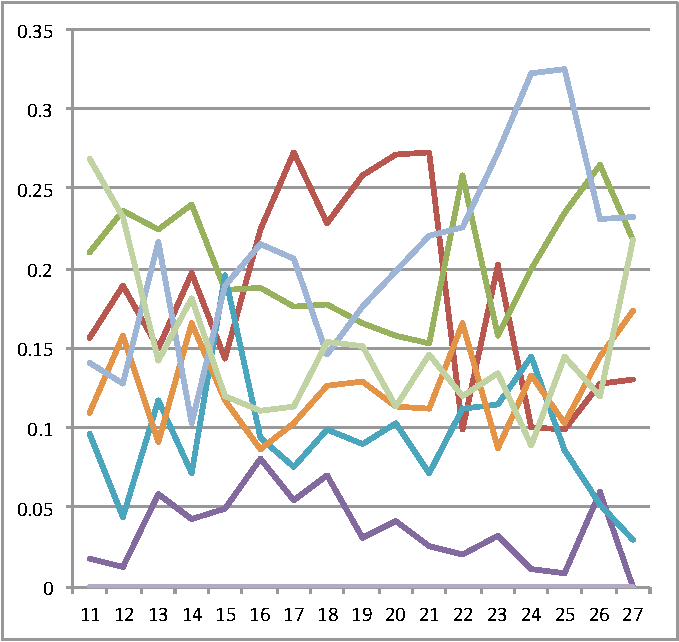
\includegraphics[width=0.48\linewidth]{figures/3LDA2TweetsInSt.pdf}
\label{fig:tweets_topics_inst}
}
\subfigure[Out of \stlouis]
{
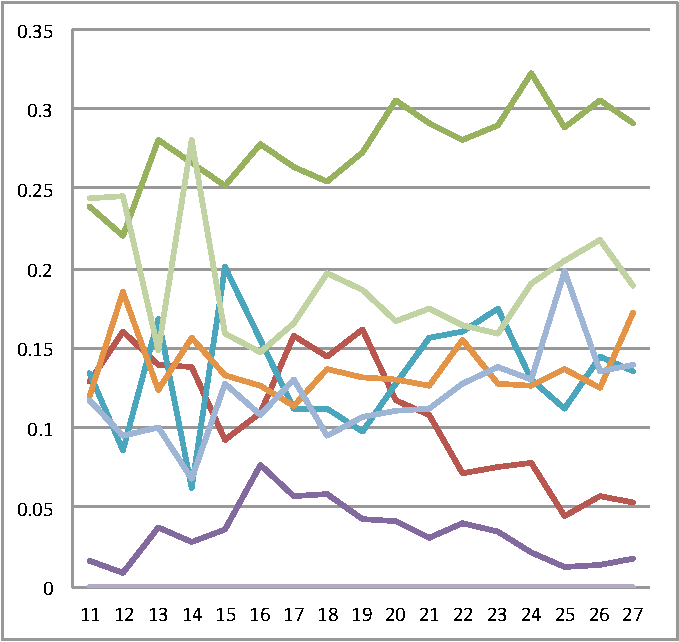
\includegraphics[width=0.48\linewidth]{figures/3LDA2TweetsOutSt.pdf}
\label{fig:tweets_topics_outst}
}
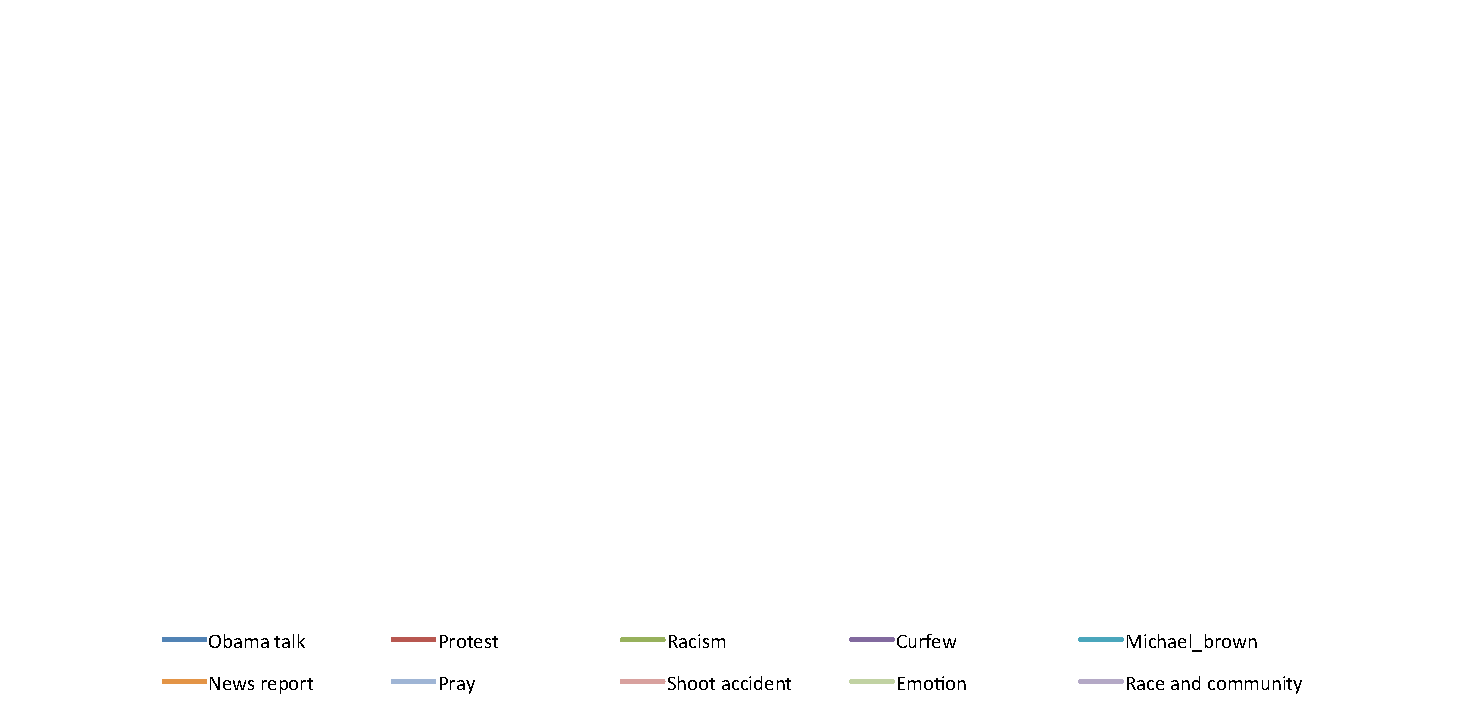
\includegraphics[width=\linewidth]{figures/Legend.pdf}
\caption{Tweets Topic Dynamics in and out of \stlouis by \stlda}\label{fig:tweets_topics_stlouis}
\end{figure*}

The proportion of tweets talking about \emph{Curfew} increases to 7.5\%, which is a peak on August 18 and then decreases. This topic change is similar for both tweets in and out of \stlouis area. Meanwhile the proportion of tweets talking about \emph{News Report} and \emph{Michael Brown} are similar along the time. Tweets about \emph{News Report} keep taking about 10\% to 15\% of all tweets. There are three small peaks on August 12, 14 and 22. Proportion of tweets talking about \emph{Michael Brown} and emph{Shoot Accident} increases a lot on August 15 in and out Ferguson area. It may be caused by the release of video recording Brown in a robbery prior to being shot. The public, both in and out of Ferguson area can be affected by it and begin to discuss a lot about it.

Difference lies in topic proportion of \emph{Pray}, but they share similar dynamics. Both in and out of \stlouis area, the increase of tweets with \emph{Pray} topic is consistent with the time when Michael Brown's funeral is held. On August 25, more than 35\% of tweets in Ferguson are about \emph{Pray}. Out of \stlouis, the number of tweets about \emph{Pray} increases to a peak on that day, taking 20\% of all.

It is reasonable to find that more tweets in \stlouis talk about \emph{Protest}, while out of \stlouis more tweets talk about \emph{Racism}. From August 18, when Governor Nixon deployed the National Guard to Ferguson, to August 21 when the National Guard withdrew, protests and conflicts keep occurring. People in Ferguson area are closer and more related to protests, so tweets with this topic surge to take more than 25\% of all tweets. Meanwhile proportion of \emph{Protest} tweets out of \stlouis is far less. The public who are not involved in the event tend to have less knowledge about real situations, but according to what they hear and know, they are better at abstract thinking about this event, thus \emph{Racism} takes majority in most of the time.

An interesting phenomenon is the \emph{Emotion} topic change. Michael Brown was killed on August 9, and anger emotion is the major topic of tweets in \stlouis, then \emph{Emotion} tweets keep decreasing, taking 10\% to 15\% of all tweets. However outside \stlouis area, there is a lag effect of \emph{Emotion} explosion. It is possible that news takes time to spread and the public outside Ferguson need more information to understand what happened. Besides, outsiders may care more about the conflicts between protesters and police, so their emotion was detonated when protests began.

Comparison of topic dynamics in and out of \stlouis area shows that, the public in \stlouis tends to publish tweets that are more related with evlovement of event, such as the shooting, protests and funeral. Meanwhile people out of \stlouis area has lag effect in \emph{Emotion} explosion and have more abstract perception on events, thus \emph{Racism} tweets take a majority. They share similar amount of focus on \emph{News Reports}, investigation of \emph{Michael Brown Shooting Accident} and \emph{Curfew}, which might because these issues are not quite closely related to them, or the influence is relatively small.

\subsection{Are Topic Dynamics of Tweets Similar with News?}

Using the results of \stlda, we compare the topics of news and tweets both in and out of \stlouis area. We observe that the three main topics in news, \emph{Obama Talk}, \emph{Shoot Accident} and \emph{Race and Community}, do not exist in tweets. However corresponding to shoot accident investigation, there is similar topic \emph{Michael Brown}, which is a main topic in tweets, taking a small proportion in news. Although the thing news and tweets talk about is the same, how they talk and what words they use is quite different, so it is identified with two separate topics for news and tweets. Similarly, \emph{Racism} topic exists mostly in tweets, while \emph{Race and Community} mainly exists in news. Although these two topics are talking about race, there is little overlapping of tweets and news in the two topics. It indicates that media and the public are using quite different words to discuss the same thing. One possible reason is that tweets use more oral language, while news uses more formal written language. It is also possible that media and the public describe the same thing with different frames. According to the top words in two topics, there are more negative words in \emph{Racism} such as \emph{stop}, \emph{riot}. In the topic labeled with \emph{Race and Community}, words like \emph{make}, \emph{good}, \emph{community} are indicative of positive emotion. Thus the public tends to have negative emotion about race issues during the Ferguson unrest, but the media tried to describe and lead the discussion to a positive way.

Two topics in tweets have little proportion in news, which are \emph{Emotion} and \emph{Prays}. It is reasonable that tweets are more subjective and contain more words about feelings, emotions and prays, while news is more serious and should be objective, avoiding emotional leadings. So the topic difference in tweets and news reflects the characteristics of two types of documents.

Another difference in news and tweets is topic diversity. Comparing topic dynamics of news (Figure~\ref{fig:news_topics_stlda}) and that of tweets (Figure~\ref{fig:tweets_topics_stlda}), it is obvious that tweets have more diverse topics, and proportion of different topics changes overtime. But there are only three main themes in news, and the changing of topics is rare. Topic related with Obama keeps a stable proportion in news report, while the report of investigation, and discussion of race issues keeps alternating dominance. The results show that public topics change along with evolvement of events, while media has certain issues to cover. Public opinions are more diverse. Under certain issues, voice of certain topic could become mainstream.

In general, the influence of media on the public is not obvious according to topic dynamics of news and tweets. Although they both concern with shoot accident and racism issues, how they talk is different. Besides there is not much similarity between topic dynamics of the two, even considering time lag. News have mainstream topics, but topics in tweets are more diverse, and evolve along with development of the event. The media care more about investigation of the shoot accident, reaction of the government and discussion of racism, but less about protests and emotion of the public. To large extent, the results support the theory of cascade model by ~\newcite{entman1993framing} from the perspective of the role media play, however the public do not shown to be heavily influenced by media frames.

\subsection{Relation between Topic Dynamics of Tweets and News}
Meanwhile we examine the common topics in news and tweets to see whether there is interaction between news and tweets. Although the common topics take a small proportion in both news and tweets. The overlapping topics are \emph{Protest}, \emph{Curfew}, \emph{Michael Brown} and \emph{News Report}, which are shown in Figure~\ref{fig:topics_news_tweets}. We compare dynamics of these topics for news and tweets separately in and out of \stlouis area. For better observation of trend, we use smoothed line here instead of linear connection between points. The topic dynamic shapes for \emph{Protest} of news and tweets seem to be similar. \emph{Protest} has peaks on almost the same day for three sets of document, while \emph{Curfew} peak in news seems to have a slight lag after tweets. It is possible that people in Ferguson are under curfew and reporting it timely, but news may take some time to process information and publish.\psrcomment{Dynamic Time Warping (DTW) would be an interesting way to look at this.}

\begin{figure*}[htpb]
\centering
\subfigure[Protest]
{
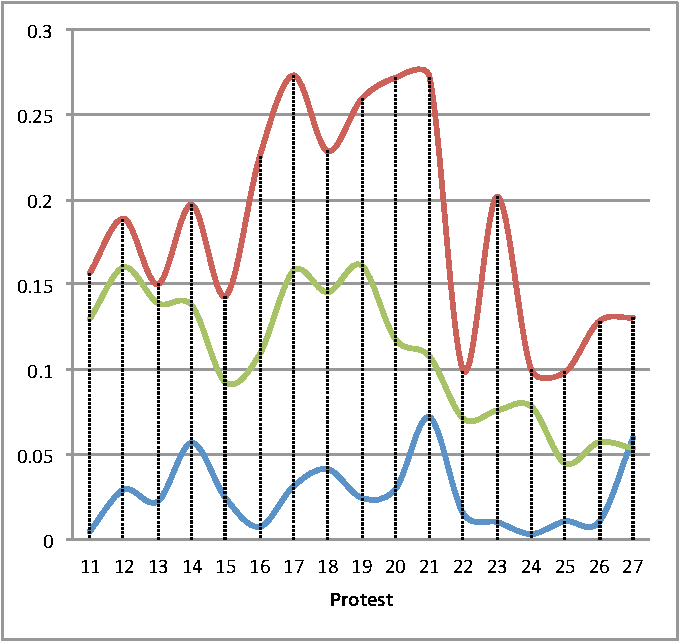
\includegraphics[width=0.48\linewidth]{figures/4_1_Protest.pdf}
\label{fig:protest}
}
\subfigure[Curfew]
{
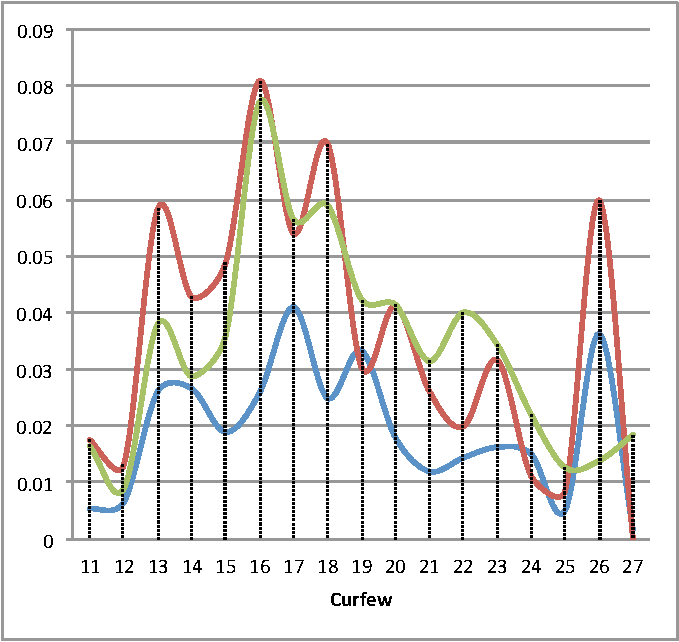
\includegraphics[width=0.48\linewidth]{figures/4_2_Curfew.pdf}
\label{fig:curfew}
}
\subfigure[Michael Brown]
{
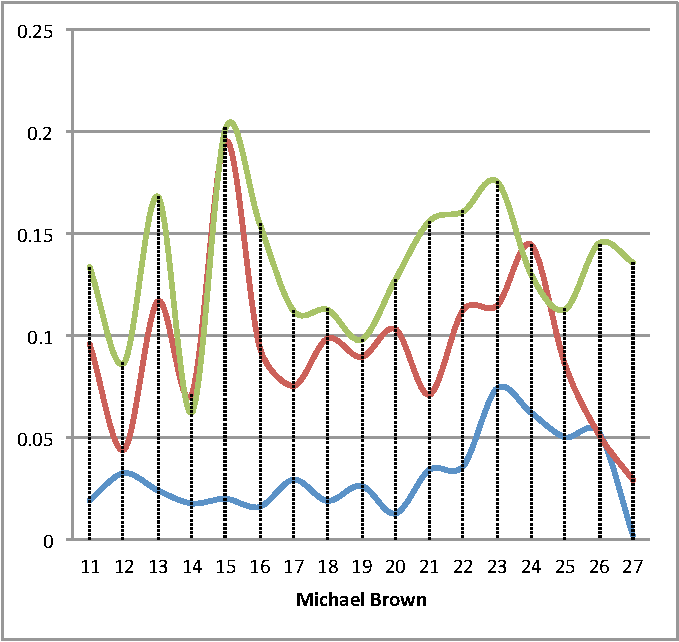
\includegraphics[width=0.48\linewidth]{figures/4_3_Michael_Brown.pdf}
\label{fig:mb}
}
\subfigure[News Report]
{
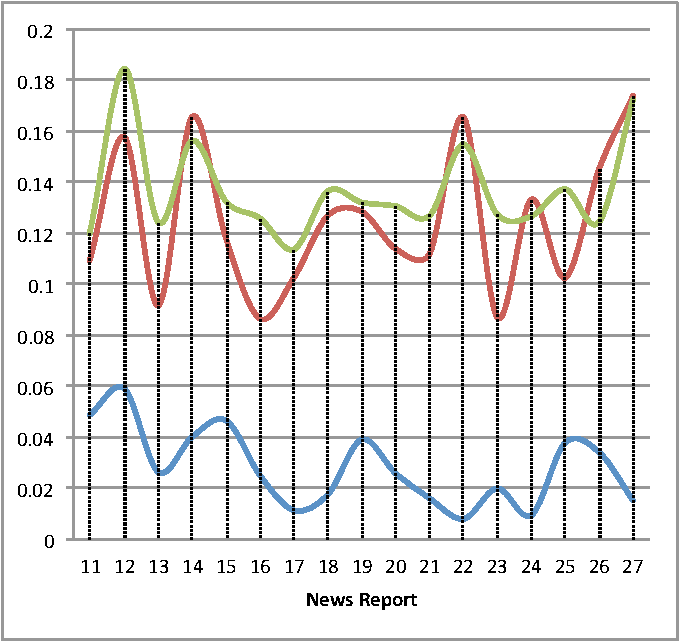
\includegraphics[width=0.48\linewidth]{figures/4_4_News_report.pdf}
\label{fig:news_report}
}
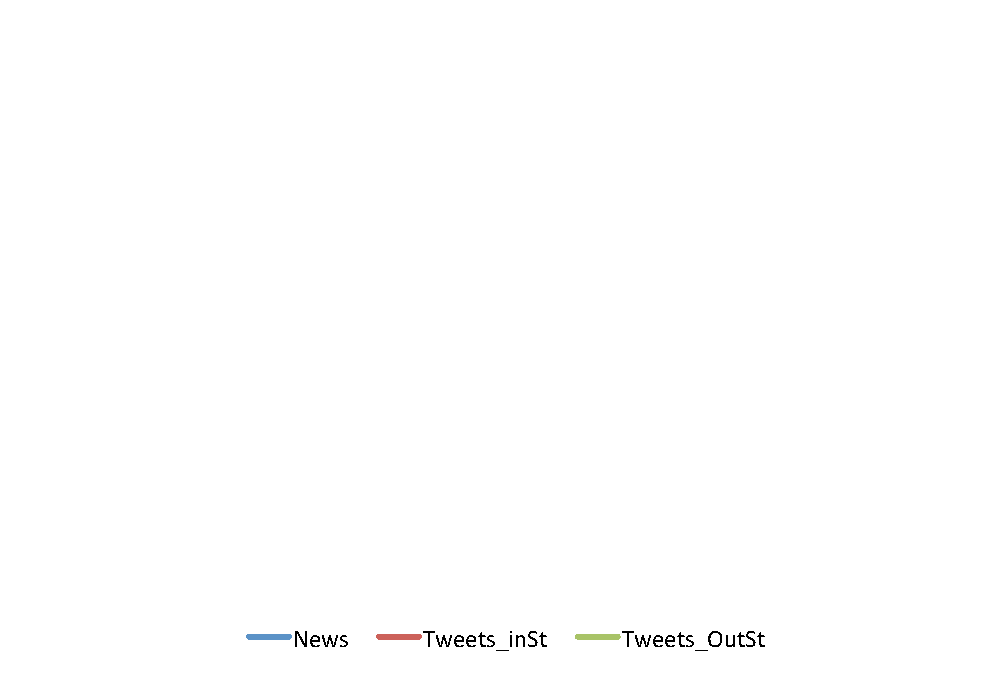
\includegraphics[width=0.5\linewidth]{figures/4_Legend_cut.pdf}
\caption{Topic Dynamic of News and Tweets by \stlda}\label{fig:topics_news_tweets}
\end{figure*}

There is no common pattern in \emph{Michael Brown}. According to analysis above, news mainly focus on investigation and getting to the bottom of shoot accident, which is labeled \emph{Shoot Accident}. It is talking about the same thing as topic \emph{Michael Brown}, however the words they use are quite different. So \emph{Michael Brown} topic has a tiny proportion in news, which takes less than 5\%.

For the topic \emph{News Report}, there is time difference in peaks of topic for news and tweets. However it is hard to know whether tweets cite some report first, and media is influenced to cite report, or in the other way around, or there may be no relation at all. 

\section{Conclusions}
\label{sec:conclu}

We propose a new topic model \stlda to discover topics in news and tweets under a unified frame. Different from conventional LDA, \stlda assigns multiple topics to news while gives only one topic to each tweet. Compared to the results of LDA, topic analysis of tweets shows that the topic given by \stlda can usually accurately summarize the topic of tweets, while LDA usually gives much more irrelevant topics. We also examine the topic dynamics of news and tweets based on results of LDA and \stlda, finding that more diverse topic changes in news can be discovered by \stlda. Moreover, topic dynamics in tweets discovered by \stlda has patterns consistent with real events. It turns out that \stlda has advantage in accurate identification of one topic for each tweet, thus avoiding the representation of noisy topics, which is usually the case in conventional LDA on tweets.

Using topics discovered by \stlda, we compare topic dynamics of tweets in and out of \stlouis area, finding that people in \stlouis area publish more about what happened in the area, and their topics are highly related with event evolvement in Ferguson. However people outside \stlouis area discuss more about the concepts such as \racism, which are abstract perception of Ferguson unrest event. Tweets in and out of Ferguson area share similar topics in \newsreport, \curfew, \shootincident and \michaelbrown.

Comparison of topic dynamics of tweets and news shows that topics in tweets are more diverse than topics in news. News and tweets both talk about the \shootincident and \racism, however \stlda identifies them as separate topics for tweets and news. From the top words in topics we find that though they describe the same event, they are using different vocabulary, which means there is much difference in how media and public talk. On the other hand, media and the public share some common topics such as \protest and \newsreport, but it is hard to identify the direction of influence considering the complicated changes of topics.

In the next step, we want to further find the relation between tweets and news, thus linking them together according to users' behaviors such as retweeting and reply. Social network is another factor that may have influence on how people think and talk about things. Incorporating social links between users is another direction for further understanding why there is the dynamics of topics.

\psrcomment{Overall nice work, and I like the way you laid out the issues and potential contributions in Section 1-2. I don't feel like you achieved the full scope of what you were aiming for, in terms of the question in introduction, but this was reasonable as an initial foray and the qualitative discussion is promising. I think the modeling using a \emph{single} topic space is what's most important and your model does seem to allow both short and long texts to co-exist with the same topics. I don't understand, though, how the full model works, since you seem only to have described the model for tweets in Section 3.}

\psrcomment{An idea to consider: rather than a categorical distribution between tweets (one topic) and news (a distribution), what about a model that selects the ``concentration" of topics based on the document length?}


\section*{Acknowledgement}

The authors would like to thank Prof. Philip Resnik and fellows in LING848 for useful advice.

\bibliographystyle{style/aaai}
\bibliography{bib/journal-full,bib/ref}

%\begin{appendix}

\section{Derivation of ST-LDA Gibbs Sampling Equation}
\label{sec:derivation}

The probability of documents over topics are computed as

\begin{eqnarray}
&&\prob{\bm{z}}{\alpha} \notag \\
&\propto& \int \prob{\bm{z}}{\bm{\theta}} \prob{\bm{\theta}}{\alpha} \mathrm{d}\bm{\theta}\\
&\propto& \int \left( \prod_{k=1}^{K} \theta_k^{N_k} \right) \left( \frac {1} {\Delta(\alpha)} \prod_{k=1}^{K} \theta_k^{\alpha-1} \right) \mathrm{d}\bm{\theta}\\
&\propto& \int \frac{1}{\Delta(\alpha)} \prod_{k=1}^{K} \theta_k^{N_k+\alpha-1} \mathrm{d}\bm{\theta}\\
&\propto& \frac{\Delta(\bm{N}+\alpha)}{\Delta(\alpha)},
\end{eqnarray}
where $\Delta(\cdot)$ is defined as

\begin{equation}
\Delta(\bm{x}) = \frac {\prod_{k=1}^{K} \Gamma(x_k)} {\Gamma(\sum_{k=1}^{K} x_k)}.
\end{equation}

The probability of words over topics are computed as

\begin{eqnarray}
&&\prob {\bm{w}} {\bm{z}, \beta} \notag \\
&\propto& \int \prob {\bm{w}} {\bm{z}, \bm{\phi}} \prob {\bm{\phi}} {\beta} \mathrm{d} \bm{\phi}\\
&\propto&\int \left( \prod_{k=1}^{K} \prod_{v=1}^{V} \phi_{k,v}^{N_{k,v}} \right) \left( \prod_{k=1}^{K} \frac {1} {\Delta(\beta)} \prod_{v=1}^{V} \phi_{k,v}^{\beta-1} \right) \mathrm{d} \bm{\phi}\\
&\propto&\int \prod_{k=1}^{K} \frac {1} {\Delta(\beta)} \prod_{v=1}^{V} \phi_{k,v}^{N_{k,v}+\beta-1} \mathrm{d} \bm{\phi}\\
&\propto&\prod_{k=1}^{K} \frac {\Delta(\bm{N_k}+\beta)} {\Delta(\beta)}.
\end{eqnarray}

Therefore, the joint probability of words and topic assignments is 

\begin{equation}
\prob {\bm{w}, \bm{z}} {\alpha, \beta} = \frac {\Delta(\bm{N}+\alpha)} {\Delta(\alpha)} \prod_{k=1}^{K} \frac {\Delta(\bm{N_k}+\beta)} {\Delta(\beta)}.
\end{equation}

Finally the Gibbs sampling equation is derived as

\begin{eqnarray}
&&\prob {z_{d}=k} {\bm{z_{-d}},\bm{w_d}} \notag \\
&\propto& \frac {\Delta(\bm{N}+\alpha)} {\Delta(\bm{N^{-d}}+\alpha)} \frac {\Delta(\bm{N_k}+\beta)} {\Delta(\bm{N_k^{-d}}+\beta)}\\
&\propto& \frac {\Gamma(N_k+\alpha)} {\Gamma(N_k^{-d}+\alpha)} \frac {\Gamma(N_{\cdot}^{-d}+K\alpha)} {\Gamma(N_{\cdot}+K\alpha)} \notag \\
&&\frac {\Gamma(N_{k,\cdot}^{-d}+V\beta)} {\Gamma(N_{k,\cdot}+V\beta)} \prod_{v=1}^{V} \frac {\Gamma(N_{k,v}+\beta)} {\Gamma(N_{k,v}^{-d}+\beta)}\\
&\propto& \frac {N_{k}^{-d}+\alpha} {N_{\cdot}^{-d}+K\alpha} \frac {\prod\limits_{v=1}^{V} \prod\limits_{i=0}^{N_{d,v}-1} (N_{k,v}^{-d}+\beta+i)} {\prod_{i=0}^{N_{d,\cdot}-1} (N_{k,\cdot}^{-d}+V\beta+i)}\\
&\propto& \left( N_{k}^{-d}+\alpha \right) \frac {\prod\limits_{v=1}^{V} \prod\limits_{i=0}^{N_{d,v}-1} (N_{k,v}^{-d}+\beta+i)} {\prod_{i=0}^{N_{d,\cdot}-1} (N_{k,\cdot}^{-d}+V\beta+i)}.
\end{eqnarray}

\end{appendix}

\end{document}
